
\documentclass{ximera}

\input{../preamble.tex}

\title{6.2 - Concavity and Inflection Points}
\outcome{State the Second Derivative Test.}
\outcome{Apply the Second Derivative Test.}
\outcome{Define inflection points.}
\outcome{Find inflection points.}
\begin{document}
\begin{abstract} \end{abstract}
\maketitle
In the previous section, we examined how we can use the first derivative to determine the shape of the graph of a function. But more information can be gained by considering the second derivative. 

\section{Inflection points}

If we are trying to understand the shape of the graph of a function,
knowing where it is concave up and concave down helps us  get a more
accurate picture. It is worth summarizing what we have already seen into
 a single theorem.

\begin{theorem}[Test for Concavity]\index{concavity test}
Suppose that $f''(x)$ exists on an interval.
\begin{enumerate}
\item If $f''(x)>0$ on an interval, then $f$ is concave up on that interval.
\item If $f''(x)<0$ on an interval, then $f$ is concave down on that interval.
\end{enumerate}
\end{theorem}


Of particular interest are points at which the concavity changes from
up to down or down to up. 

\begin{definition}\index{inflection point}
If $f$ is continuous at $x=a$ and its concavity changes either from up to down
or down to up at $x=a$, then $f$ has an \dfn{inflection point} at
$x=a$.
\end{definition}

It is instructive to see some examples of inflection points:
\begin{image}
\begin{tikzpicture}
	\begin{axis}[
            %height=7cm,
            %width=2in,
            width=6in,
            height=2in,
            %ymax=8,
            %ymin=-1,
            axis lines=none,
            clip=false,
          ]
          \addplot [very thick, penColor, smooth, domain=(0:1)] {(x-1)^2+1};
          \addplot [very thick, penColor, smooth, domain=(1:2)] {-(x-1)^2+1};
          \addplot[color=penColor,fill=penColor,only marks,mark=*] coordinates{(1,1)};
          \node at (axis cs:1,-.5) [text width=2in] {This is an inflection point. The concavity changes from concave up to concave down.};
        
          \addplot [very thick, penColor, smooth,domain=(4:5)] {-sqrt(abs(1-(x-4)))+1};
          \addplot [very thick, penColor, smooth,domain=(5:6)] {sqrt((x-4)-1)+1};
          \addplot[color=penColor,fill=penColor,only marks,mark=*] coordinates{(5,1)};
          \node at (axis cs:5,-.5) [text width=2in] {This is an inflection point. The concavity changes from concave up to concave down.};
        \end{axis}
\end{tikzpicture}
\end{image}

It is also instructive to see some nonexamples of inflection points:
\begin{image}
\begin{tikzpicture}
	\begin{axis}[
            %height=7cm,
            %width=2in,
            width=6in,
            height=2in,
            %ymax=8,
            %ymin=-1,
            axis lines=none,
            clip=false,
          ]
          \addplot [very thick, penColor2, smooth, domain=(0:2)] {-(x-1)^2+1};
          \addplot[color=penColor2,fill=penColor2,only marks,mark=*] coordinates{(1,1)};
          \node at (axis cs:1,-.5) [text width=2in] {This is \textbf{not} an inflection point. The curve is concave down on either side of the point.};
          \addplot [very thick, penColor2, smooth,domain=(4:5)] {sqrt(abs(1-(x-4)))};
          \addplot [very thick, penColor2, smooth,domain=(5:6)] {sqrt(x-5)};
          \addplot[color=penColor2,fill=penColor2,only marks,mark=*] coordinates{(5,0)};
          \node at (axis cs:5,-.5) [text width=2in] {This is \textbf{not} an inflection point. The curve is concave down on either side of the point.};
        \end{axis}
\end{tikzpicture}
\end{image}

We identify inflection points by first finding $x$ such that $f''(x)$
is zero or undefined and then checking to see whether $f''(x)$ does in
fact go from positive to negative or negative to positive at these
points.

\begin{warning}
Even if $f''(a) = 0$, the point determined by $x=a$ might \textbf{not}
be an inflection point.
\end{warning}
\begin{example}
Describe the concavity of $f(x)=x^4$. 

\begin{explanation}
To start, compute the first and second derivative of $f(x)$ with
respect to $x$,
\[
f'(x)=\answer[given]{4x^3}\qquad\text{and}\qquad f''(x)=\answer[given]{12x^2}.
\]

Since $f''(0)=0$, there is potentially an inflection point at
$x=0$. But, for any  $x\ne 0$, $f''(x)>0$. Hence there is no inflection point at $x=0$. The curve is
concave up for all $x<0$ and  remains concave up for all $x>0$.
\end{explanation}
\end{example}
\begin{example}
Describe the concavity of $f(x)=x^3-x$. 

\begin{explanation}
To start, compute the first and second derivative of $f(x)$ with
respect to $x$,
\[
f'(x)=\answer[given]{3x^2-1}\qquad\text{and}\qquad f''(x)=\answer[given]{6x}.
\]
Since $f''(0)=0$, there is potentially an inflection point at
$x=0$. Using test points, we note the concavity does change from down
to up, hence there is an inflection point at $x=0$. The curve is
concave down for all $x<0$ and concave up for all $x>0$, see the
graphs of $f(x) = x^3-x$ and $f''(x) = 6x$.
\begin{image}
\begin{tikzpicture}
	\begin{axis}[
            domain=-3:3,
            ymax=3,
            ymin=-3,
            axis lines =middle, xlabel=$x$, ylabel=$y$,
            every axis y label/.style={at=(current axis.above origin),anchor=south},
            every axis x label/.style={at=(current axis.right of origin),anchor=west}
          ]
          \addplot [very thick, penColor, smooth] {x^3-x};
          \addplot [very thick, penColor4, smooth] {6*x};         
          \node at (axis cs:-.75,.6) [anchor=west] {\color{penColor}$f$};  
          \node at (axis cs:.2,1) [anchor=west] {\color{penColor4}$f''$};
          \addplot[color=penColor4!50!penColor,fill=penColor4!50!penColor,only marks,mark=*] coordinates{(0,0)};  %% closed hole
        \end{axis}
\end{tikzpicture}
%% \caption{A plot of $f(x) = x^3-x$ and $f''(x) = 6x$. We can see that
%%   the concavity change at $x=0$.}
%% \label{figure:3x^2-1}
%% \end{marginfigure}
\end{image}
\end{explanation}
\end{example}


Note that we need to compute and analyze the second derivative to
understand concavity. But that is not the only way we can use the second derivative! We can also use it to determine the location for maxima and minima. As a note, if for some reason this fails
we can then try one of the other tests.

\section{The second derivative test}


Recall the first derivative test:

\begin{itemize}
\item If $f'(x)>0$ for all $x$ that are near and to the left of $a$ and $f'(x)<0$  for all $x$ that are near and to the right of
  $a$, then the function $f$ has a local maximum at $a$.
\item If $f'(x)<0$ for all $x$ that are near and  to the left of $a$ and $f'(x)>0$ for all $x$ that are near and  to the right of
  $a$, then the function $f$ has a local minimum at $a$.
\end{itemize}

Assume that a function $f$ has  a critical point at $a$ and that $f'(a)=0$.
If $f'$  happens to be decreasing on some interval containing $a$, then it changes from positive to negative at $a$. 

Recall, that when $f'(x)<0$, we know that $f$ is decreasing and when $f'(x)>0$, then $f$ is increasing. We can use this same logic for $f''(x)$ and $f'(x)$.

If $f''$ is negative on some interval that contains $a$,
then $f'$ is decreasing so there is a local maximum at
the point in question. On the other hand, if $f'$ is increasing, then it changes from
negative to positive at $a$. Therefore,
if $f''$ is positive on an interval that contains $a$, then
$f'$ is increasing, so there is a local minimum at the
point in question. We summarize this as the \textit{second derivative
  test}.

\begin{theorem}[Second Derivative Test]\index{second derivative test}\label{T:sdt}
Suppose that $f''(x)$ is continuous on an open interval and that
$f'(a)=0$ for some value of $a$ in that interval.
\begin{itemize}
\item If $f''(a) <0$, then $f$ has a local maximum at $a$.
\item If $f''(a) >0$, then $f$ has a local minimum at $a$.
\item If $f''(a) =0$, then the test is inconclusive. In this case,
  $f$ may or may not have a local extremum at $x=a$.
\end{itemize}
\end{theorem}


The second derivative test is often the easiest way to identify local
maximum and minimum points. Sometimes the test fails and sometimes
the second derivative is quite difficult to evaluate. In such cases we
must fall back on one of the previous tests.

\begin{example}
Once again, consider the function 
\[
f(x) = \frac{x^4}{4}+\frac{x^3}{3}-x^2
\]
Use the second derivative test to locate the
local extrema of $f$.

\begin{explanation}
Start by computing
\[
f'(x) = \answer[given]{x^3 + x^2 -2x} \qquad\text{and}\qquad f''(x) = \answer[given]{3x^2 + 2x-2}.
\] 
Using the same technique as we used before, we find that 
\[
f'(-2) = \answer[given]{0},\qquad f'(0) = \answer[given]{0}, \qquad f'(1) = \answer[given]{0}. 
\]
Now we'll attempt to use the second derivative test,
\[
f''(-2) = \answer[given]{6}, \qquad f''(0) =\answer[given]{ -2}, \qquad f''(1) = \answer[given]{3}.
\]
Hence we see that $f$ has a local minimum at $x=-2$, a local
maximum at $x=0$, and a local minimum at $x=1$, see below for a plot
of $f(x) =\frac{x^4}{4} + \frac{x^3}{3} -x^2$ and $f''(x) = 3x^2 + 2x -2$:
\begin{image}
\begin{tikzpicture}
	\begin{axis}[
            domain=-4:4,
            ymax=7,
            ymin=-4,
            %samples=100,
            axis lines =middle, xlabel=$x$, ylabel=$y$,
            every axis y label/.style={at=(current axis.above origin),anchor=south},
            every axis x label/.style={at=(current axis.right of origin),anchor=west}
          ]
          \addplot [dashed, textColor, smooth] plot coordinates {(-2,-2.667) (-2,6)}; %% {.451};
          \addplot [dashed, textColor, smooth] plot coordinates {(1,0) (1,3)}; %% axis{2.215};

          \addplot [very thick, penColor, smooth] {(x^4)/4 + (x^3)/3 -x^2};
          \addplot [very thick, penColor4, smooth] {3*x^2 + 2*x -2};

          \node at (axis cs:-1.7,-2.7) [anchor=west] {\color{penColor}$f$};  
          \node at (axis cs:-1.5,2) [anchor=west] {\color{penColor4}$f''$};

          \addplot[color=penColor4,fill=penColor4,only marks,mark=*] coordinates{(-2,6)};  %% closed hole
          \addplot[color=penColor4,fill=penColor4,only marks,mark=*] coordinates{(1,3)};  %% closed hole
          \addplot[color=penColor4,fill=penColor4,only marks,mark=*] coordinates{(0,-2)};  %% closed hole
          \addplot[color=penColor,fill=penColor,only marks,mark=*] coordinates{(0,0)};  %% closed hole
          \addplot[color=penColor,fill=penColor,only marks,mark=*] coordinates{(-2,.-2.667)};  %% closed hole
          \addplot[color=penColor,fill=penColor,only marks,mark=*] coordinates{(1,-.4167)};  %% closed hole
        \end{axis}
\end{tikzpicture}
%% \caption{A plot of $f(x) =x^4/4 + x^3/3 -x^2$ and $f''(x) = 3x^2 + 2x -2$.}
%% \label{figure:SDT(x^4)/4 + (x^3)/3 -x^2}
\end{image}

\end{explanation}
\end{example}


\begin{question}
  If $f''(a)=0$, what does the second derivative test tell us?
  \begin{multipleChoice}
    \choice{The function has a local extremum at $x=a$.}
    \choice{The function does not have a local extremum at $x=a$.}
    \choice[correct]{It gives no information on whether the function has a local extremum at $x=a$.} 
  \end{multipleChoice}

\end{question}
Let's put together all of the information we've discussed in a single problem.

\begin{example}
    Consider the function $f(x)=x^4-4x^3$. Determine the intervals of increase and decrease, local maximum and minimum values, intervals of concavity, and inflection points.
\begin{explanation}
    Let's start by finding the first and second derivatives of our function with respect to x.
    \[f'(x)=\answer[given]{4x^3-12x^2}\]
    \[f''(x)=\answer[given]{12x^2-24x}\]

Let's start by working with the first derivative and finding the critical values of $y$. Let's start by factoring $y'$ and setting it equal to zero,
\[f'(x)=4x^3-12x^2=\answer[given]{4x^2}(x-3)=0.\]

We can see that the critical values of $f(x)=x^4-4x^3$ are $x=\answer[given]{0}$ and $x=3$.

We will start by setting up a sign table
\begin{figure}[h!]
    \centering
 

\begin{tikzpicture}
\tkzTabInit[lgt=4,espcl=2,deltacl=0]
  { /.8, $4x^2$ /.8, $x-3$ /.8, $f'(x)=4x^2(x-3)$ /.8}
  {,$0$,$3$,} % four main references
\tkzTabLine {,,t,,t,,} % seven denotations
\tkzTabLine {,,t,,t,,}
\tkzTabLine {,,t,,t,,}
\end{tikzpicture}
\end{figure}

We need to choose a point that exists in each interval. We will use $x=-1$ from $(-\infty,0)$, $x=1$ from $(0,3)$, and $x=4$ from $(3,\infty)$. However, you can use any point that you want as long as each point lies in the appropriate interval. We will then plug those values into $f'(x)$ and record that information in a sign table. 

\begin{figure}[h!]
    \centering
 

\begin{tikzpicture}
\tkzTabInit[lgt=4,espcl=2,deltacl=0]
  { /.8, $4x^2$ /.8, $x-3$ /.8, $f'(x)=4x^2(x-3)$ /.8}
  {,$0$,$3$,} % four main references
\tkzTabLine {,+,z,+,t,+,} % seven denotations
\tkzTabLine {,-,t,-,z,+,}
\tkzTabLine {,-,z,-,z,+,}
\end{tikzpicture}
\end{figure}

This shows us that $f(x)=x^4-4x^3$ is increasing on the interval $(\answer[given]{3},\infty)$ and decreasing on the interval $(-\infty,\answer[given]{0})\cup(0,\answer[given]{3})$.

Further, from this diagram, we can see that $f(x)$ changes from decreasing to increasing around $x=3$. Thus we have a local minimum at the point $(3,f(3))=(3,\answer[given]{-27})$. Notice that there are no local maximums since the derivative does not change from increasing to decreasing around any of our critical points.

Now we move on to concavity and inflection points which requires us to use the second derivative, $f''(x)=12x^2-24x$. We can start by factoring our second derivative and setting it equal to 0.
\[f''(x)=12x^2-24x=12x(\answer[given]{x-2})=0.\]
Solving, we get critical points for $f'(x)$ as $x=0$ and $x=\answer[given]{2}$.

Putting together a sign table, we get:
\begin{figure}[h!]
    \centering
\begin{tikzpicture}
\tkzTabInit[lgt=4,espcl=2,deltacl=0]
  { /.8, $12x$ /.8, $x-2$ /.8, $f''(x)=12x(x-2)$ /.8}
  {,$0$,$2$,} % four main references
\tkzTabLine {,,t,,t,,} % seven denotations
\tkzTabLine {,,t,,t,,}
\tkzTabLine {,,t,,t,,}
\end{tikzpicture}
\end{figure}
Now we need to select a point in each of the three intervals, $(-\infty,0), (0,2),$ and $(2,\infty)$. We will use $x=-1, x=1,$ and $x=3$ respectively. Filling in the sign table with that in mind.
\begin{figure}[h!]
    \centering
\begin{tikzpicture}
\tkzTabInit[lgt=4,espcl=2,deltacl=0]
  { /.8, $12x$ /.8, $x-2$ /.8, $f''(x)=12x(x-2)$ /.8}
  {,$0$,$2$,} % four main references
\tkzTabLine {,-,z,+,t,+,} % seven denotations
\tkzTabLine {,-,t,-,z,+,}
\tkzTabLine {,+,z,-,z,+,}
\end{tikzpicture}
\end{figure}
So that means that our function, $f(x)=x^4-4x^3$ is concave up on the interval $(\infty,0)\cup(\answer[given]{2},\infty)$ and concave down on the interval $(\answer[given]{0}, \answer[given]{2})$.

We can see that our function changes concavity around $x=0$ and $x=2$ so that means that we have an inflection point at each of these. Thus, our inflection points are at $(0,f(0))=(0,\answer[given]{0})$ and $(2,f(2))=(2,\answer[given]{-16})$.
\end{explanation}
\end{example}
\end{document}